\begin{frame}[fragile]{Inheritance}
  \vfill
  \begin{lstlisting}[firstnumber=2]
class Figura {
protected:
  int b, h;
public:
  Figura();
  void set_data(int,int);
};
...\end{lstlisting}
  \vfill
  \begin{itemize}
    \item Classe di base con certe caratteristiche
    \vfill
    \item \lstinline$protected$, alternativa a \lstinline$private$/\lstinline$public$
    \begin{itemize}
      \item membri \lstinline$protected$ sono inaccessibili dall'esterno
      \item possono essere \alert{ereditati}
    \end{itemize}
  \end{itemize}
  \vfill
\end{frame}

\begin{frame}[fragile]{Inheritance}
  \vfill
  \begin{lstlisting}[firstnumber=13]
...
Figura::Figura() { return; }
void Figura::set_data(int b, int h) {
  this->b = b;
  this->h = h;
  return;
}
...\end{lstlisting}
  \vfill
  \begin{itemize}
    \item Implementazione delle funzioni
  \end{itemize}
  \vfill
\end{frame}

\begin{frame}[fragile]{Inheritance}
  \vfill
  \begin{lstlisting}[firstnumber=8]
...
class Rett : public Figura {
public:
  Rett();
  int area() const;
};
...\end{lstlisting}
  \vfill
  \begin{itemize}
    \item Classe \alert{derivata}
    \begin{itemize}
      \item eredita tutti i membri \lstinline$public$ o \lstinline$protected$
      \item i membri \lstinline$private$ non vengono ereditati
    \end{itemize}
    \vfill
    \item I costruttori devono essere ridefiniti
    \begin{itemize}
      \item il nome del vecchio costruttore è diverso
    \end{itemize}
  \end{itemize}
  \vfill
\end{frame}

\begin{frame}[fragile]{Inheritance}
  \vfill
  \begin{lstlisting}[firstnumber=19]
...
Rett::Rett() { return; }
int Rett::area() const{
  return this->b*this->h;
}
...\end{lstlisting}
  \vfill
  \begin{itemize}
    \item Implementazione delle funzioni
    \vfill
    \item Non è necessario reimplementare \lstinline$set_data$
  \end{itemize}
  \vfill
\end{frame}

\begin{frame}[fragile]{Inheritance}
  \vfill
  \begin{lstlisting}[firstnumber=23]
...
int main() {
  Rett a;
  a.set_data(3,5);
  std::cout << "Area = " << a.area() << std::endl;
  return 0;
}
...\end{lstlisting}
  \vfill
  \begin{itemize}
    \item Utilizzo nel programma
  \end{itemize}
  \vfill
\end{frame}

\begin{frame}[fragile]{Inheritance}
  \vfill
  \begin{itemize}
    \item Una classe può ereditare da più fonti
    \begin{itemize}
      \item \lstinline$class Derivata : public Fonte1, public Fonte2$
    \end{itemize}
    \vfill
    \item L'eredità può modificare gli accessi
    \begin{itemize}
      \item \lstinline$class Derivata : public Fonte$
      \item \lstinline$class Derivata : protected Fonte$
      \item \lstinline$class Derivata : private Fonte$
    \end{itemize}
    \vfill
    \item L'eredità è alla base di una buona OOP
  \end{itemize}
  \vfill
\end{frame}

\begin{frame}[fragile]{Templates}
  \vfill
  \begin{lstlisting}
#include <iostream>
template<class T> T max(const T,const T);
int main(){
  std::cout << max<int>(4,5) << std::endl;
  return 0;
}
template<class T> T max(const T a,const T b) {
  T c;
  if (a >= b) { c = a; }
  else { c = b; }
  return c;
}
  \end{lstlisting}
  \vfill
  \begin{itemize}
    \item Un \alert{template} permette di creare funzioni o classi basate su classi generiche
  \end{itemize}
  \vfill
\end{frame}

\begin{frame}[fragile]{Array}
  \vfill
  \begin{center}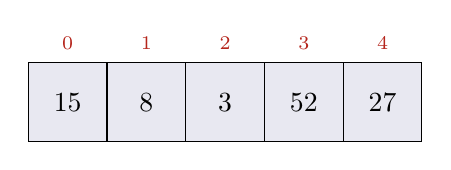
\begin{tikzpicture}
    \filldraw[fill=MidnightBlue!10!white] (0,0) rectangle ++(1,1)
                                          (1,0) rectangle ++(1,1)
                                          (2,0) rectangle ++(1,1)
                                          (3,0) rectangle ++(1,1)
                                          (4,0) rectangle ++(1,1);
    \path (0.5,0.5) node {15}
          (1.5,0.5) node {8}
          (2.5,0.5) node {3}
          (3.5,0.5) node {52}
          (4.5,0.5) node {27};
    \path[BrickRed] (0.5,1.25) node {\scriptsize 0}
                    (1.5,1.25) node {\scriptsize 1}
                    (2.5,1.25) node {\scriptsize 2}
                    (3.5,1.25) node {\scriptsize 3}
                    (4.5,1.25) node {\scriptsize 4};
  \end{tikzpicture}\end{center}
  \vfill
  \begin{itemize}
    \item Un \alert{array} è una struttura che può contenere una serie di valori,
    indicizzati da un numero intero
    \vfill
    \item In \CC\ l'indice parte sempre da 0
  \end{itemize}
  \vfill
\end{frame}

\begin{frame}[fragile]{Array}
  \vfill
  \begin{lstlisting}
#include <iostream>
#include <array>
int main(){
  std::array<int,5> a;
  for(std::size_t i = 0; i < a.size(); i++) {
    a.at(i) = 2*i;
    std::cout << a.at(i) << std::endl;
  }
  return 0;
}
  \end{lstlisting}
  \vfill
  \begin{itemize}
    \item Necessario includere l'header \lstinline$<array>$
    \vfill
    \item \lstinline$std::array$ è un template con due parametri
    \begin{itemize}
      \item il primo dice il tipo di dato contenuto
      \item il secondo dice il numero di celle
    \end{itemize}
  \end{itemize}
  \vfill
\end{frame}

\begin{frame}[fragile]{Array}
  \vfill
  \begin{lstlisting}
#include <iostream>
#include <array>
int main(){
  std::array<int,5> a;
  for(std::size_t i = 0; i < a.size(); i++) {
    a.at(i) = 2*i;
    std::cout << a.at(i) << std::endl;
  }
  return 0;
}
  \end{lstlisting}
  \vfill
  \begin{itemize}
    \item \lstinline$std::size_t$ è un tipo di intero senza segno
    \begin{itemize}
      \item buona abitudine utilizzarlo nei cicli sugli array
    \end{itemize}
    \vfill
    \item \lstinline$.size()$ restituisce il numero di elementi dell'array
    \vfill
    \item \lstinline$.at(i)$ permette di accedere all'\lstinline$i$-esimo elemento
  \end{itemize}
  \vfill
\end{frame}

\begin{frame}[fragile]{Array}
  \vfill
  \begin{lstlisting}
#include <iostream>
#include <array>
int main(){
  const int n = 5;
  std::array<int,n> a;
  for(std::size_t i = 0; i < a.size(); i++) {
    a.at(i) = 2*i;
    std::cout << a.at(i) << std::endl;
  }
  return 0;
}
  \end{lstlisting}
  \vfill
  \begin{itemize}
    \item \lstinline$std::array$ accetta solo parametri costanti
    \begin{itemize}
      \item array \alert{statico}
    \end{itemize}
  \end{itemize}
  \vfill
\end{frame}

\begin{frame}[fragile]{Array}
  \vfill
  \begin{lstlisting}
#include <iostream>
#include <vector>
int main(){
  int n;
  std::cin >> n;
  std::vector<int> a(n);
  for(std::size_t i = 0; i < a.size(); i++) {
    a.at(i) = 2*i;
    std::cout << a.at(i) << std::endl;
  }
  return 0;
}
  \end{lstlisting}
  \vfill
  \begin{itemize}
    \item \lstinline$std::vector$ è un array \alert{dinamico}
    \begin{itemize}
      \item consumo leggermente maggiore di memoria
    \end{itemize}
  \end{itemize}
  \vfill
\end{frame}

\begin{frame}[fragile]{Array}
  \vfill
  \begin{lstlisting}
#include <iostream>
#include <vector>
int main(){
  int n;
  std::vector<int> a(10);
  for(std::size_t i = 0; i < a.size(); i++) {
    a.at(i) = 2*i;
    std::cout << a.at(i) << std::endl;
  }
  std::cin >> n;
  a.resize(n);
  for(std::size_t i = 0; i < a.size(); i++) {
    std::cout << a.at(i) << std::endl;
  }
  return 0;
}
  \end{lstlisting}
  \vfill
  \begin{itemize}
    \item \lstinline$.resize$ ridimensiona l'array
  \end{itemize}
  \vfill
\end{frame}

\begin{frame}[fragile]{Array}
  \vfill
  \begin{lstlisting}
#include <iostream>
int main(){
  int a[5];
  for(std::size_t i = 0; i < 5; i++) {
    a[i] = 2*i;
    std::cout << a[i] << std::endl;
  }
  return 0;
}
  \end{lstlisting}
  \vfill
  \begin{itemize}
    \item Legacy C-style array
    \begin{itemize}
      \item sconsigliato: non controlla i limiti
      \item \lstinline$a[10]$ non darebbe errore
    \end{itemize}
  \end{itemize}
  \vfill
\end{frame}

\begin{frame}[fragile]{Matematica}
  \vfill
  \begin{itemize}
    \item La libreria \lstinline$<cmath>$:
    \begin{itemize}
      \item \lstinline$std::pow(x,y)$ \( = x^y\)
      \item \lstinline$std::sqrt(x)$ \( = \sqrt{x}\)
      \item \lstinline$std::sin(x)$, \lstinline$std::cos(x)$, \lstinline$std::tan(x)$
      \item \lstinline$std::asin(x)$, \lstinline$std::acos(x)$, \lstinline$std::atan(x)$
      \item \lstinline$std::atan2(y,x)$  \( = \arctan{\frac{y}{x}}\) nel giusto quadrante
      \item \lstinline$std::exp(x)$ \( = e^x\)
      \item \lstinline$std::log(x)$ \( = \ln{x}\)
      \item eccetera...
    \end{itemize}
  \end{itemize}
  \vfill
\end{frame}

\begin{frame}[fragile]{Matematica}
  \vfill
  \begin{itemize}
    \item La libreria \lstinline$<complex>$:
    \begin{itemize}
      \item \lstinline$std::complex<double>$ tipo di dato
      \item \lstinline$std::real(x)$ \( = \Re{x}\)
      \item \lstinline$std::imag(x)$ \( = \Im{x}\)
      \item \lstinline$std::abs(x)$ \( = |x|\)
      \item \lstinline$std::arg(x)$ \( = \arg{x}\)
      \item overload di operazioni e funzioni
    \end{itemize}
  \end{itemize}
  \vfill
  \begin{lstlisting}
#include <iostream>
#include <complex>
int main(){
  std::complex<double> a(-2,0);
  std::cout << std::sqrt(a) << std::endl;
  return 0;
}
  \end{lstlisting}
  \vfill
\end{frame}

\begin{frame}[fragile]{Progetti}
  \vfill
  \begin{itemize}
    \item Gestire un progetto su più file
    \vfill
    \item Librerie: \lstinline$esempio.hpp$
    \begin{itemize}
      \item dovrebbero contenere solo le dichiarazioni
      \item incluse in altri file con \lstinline$#include "esempio.hpp"$
      \item \alert{mai} utilizzare \lstinline$using$
    \end{itemize}
    \vfill
    \item Implementazione delle librerie: \lstinline$esempio.cpp$
    \begin{itemize}
      \item contengono la definizione delle funzioni o oggetti della libreria corrispondente
    \end{itemize}
    \vfill
    \item File principale: \lstinline$progetto.cpp$
    \begin{itemize}
      \item contiene il \lstinline$main()$
    \end{itemize}
  \end{itemize}
  \vfill
\end{frame}

\begin{frame}[fragile]{Progetti}
  \vfill
  \begin{itemize}
    \item \lstinline$myheader.hpp$:
  \begin{lstlisting}
#ifndef TASSONI2016
#define TASSONI2016
int twice(int);
#endif
  \end{lstlisting}
  \vfill
    \item \lstinline$myheader.cpp$:
  \begin{lstlisting}
int twice(int x) { return 2*x; }
  \end{lstlisting}
  \vfill
    \item \lstinline$project.hpp$:
    \begin{lstlisting}
#include <iostream>
#include "myheader.hpp"
int main() {
  std::cout << twice(5) << std::endl;
}
  \end{lstlisting}
  \end{itemize}
  \vfill
\end{frame}

\begin{frame}[fragile]{Progetti}
  \vfill
  \begin{lstlisting}
#ifndef ETICHETTA
#define ETICHETTA
...
#endif
  \end{lstlisting}
  \vfill
  \begin{itemize}
    \item \alert{Include guard}: evita che lo stesso header sia incluso più volte
    se è già stato incluso tramite un altro header
    \vfill
    \item Ogni header dovrebbe avere la propria etichetta
  \end{itemize}
  \vfill
\end{frame}

\begin{frame}[fragile]{Progetti}
  \vfill
  \begin{itemize}
    \item Compilare un progetto richiede di compilare in ordine le varie parti che
    lo costituiscono
    \vfill
    \item Ogni IDE gestisce la cosa in maniera diversa
    \vfill
    \item Sistemi *nix (Linux/MacOS) supportano \alert{Makefile}
    \begin{itemize}
      \item estremamente flessibile nella gestione di progetti ampi
      \item esempio: \lstinline$CPPMakefile$
    \end{itemize}
  \end{itemize}
  \vfill
\end{frame}

\begin{frame}{Software Open Source}
  \vfill
  \begin{itemize}
    \item \alert{Free} Software
    \begin{itemize}
      \item free = libero
      \item free = gratuito
    \end{itemize}
    \vfill
    \item Software di cui il codice sorgente è
    \begin{itemize}
      \item visibile a tutti: non serve fiducia
      \item modificabile da tutti: adattabilità
    \end{itemize}
    \vfill
    \item Sviluppato da grandi comunità
    \begin{itemize}
      \item given enough eyeballs, all bugs are shallow
      \item maggiore sicurezza
      \item maggiore qualità
    \end{itemize}
    \vfill
    \item Libertà
    \begin{itemize}
      \item da logiche di mercato
      \item da controllo esterno
    \end{itemize}
  \end{itemize}
  \vfill
\end{frame}
